\documentclass[a4paper, 11pt]{report}

\usepackage[latin1]{inputenc}
\usepackage[italian]{babel}
\usepackage{makeidx}
\usepackage[pdfborder=0]{hyperref}
\usepackage{graphicx}
\usepackage{amsmath}
\usepackage{colortbl}

\title{\Huge\textbf{Elaborato\\di\\Sistemi Informativi e Servizi in Rete}\\ \vspace{1cm} \huge Negozio di vendita on-line di Magliette Personalizzate}
\author{\textit{Iora Marco} Matricola: 65574\and \textit{Lorenzi Roberta} Matricola: 72361\and \textit{Piccinelli Andrea} Matricola: 83392}
\date{A.A. 2011--2012}

\begin{document}
\begin{figure}[t]
	\centering
	
\includegraphics[height=4cm, width=4cm]{logoUnibs.jpg}\\
	Universit� degli Studi di Brescia\\Facolt� di Ingegneria\\Corso di Laurea Magistrale e di Laurea Specialistica\\ in Ingegneria Informatica
\end{figure}
\maketitle

\tableofcontents

\chapter{Analisi dei Requisiti}
\newpage

\section{Descrizione Generale del Sito}
\subsection{Scenario}
Si vuole mettere a disposizione di potenziali clienti un \textit{negozio virtuale} in cui potranno
acquistare capi di abbigliamento (magliette), seguendoli durante tutti i passi della realizzazione 
(personalizzazione delle stampe e creazione magliette, effettuare un ordine e controllo dello stesso).\\
Con questo sito, quindi, i potenziali clienti potranno sia visualizzare il catalogo delle tipologie
di magliette possibili e delle stampe presenti, sia creare o personalizzare le proprie magliette 
secondo le proprie preferenze ed esigenze con l'invio di file scelti dall'utente, sia effettuare 
l'ordine e monitorarlo fino alla consegna.\\
Questo sito � fruito anche dal personale interno all'azienda ed in particolare agli addetti allo 
stampaggio e confezionamento delle magliette. Questi potranno sia visualizzare gli ordini effettuati dai
clienti finali e prenderli in carico, sia visualizzare gli ordini gi� presi in carico e non ancora
finiti, sia evadere l'ordine (cio� affidarlo al corriere) inserendo l'identificativo di tracciabilit�
della spedizione dato dal corriere.\\
L'azienda incarica una societ� esterna per la spedizione della merce ai propri clienti.
<<<<<<< HEAD

=======
\subsection{Progettazione delle strutture dati e delle tipologie di utenti}
Il modello dei dati include:
\begin{itemize}
	\item l'azienda descritta da nome, indirizzo, partita iva, codice fiscale, ragione sociale, e-mail,
	descrizione, informazioni sulla spedizione (costi e tempi di spedizione)
	\item le magliette fra le quali l'utente potr� scegliere, descritte da nome, colore, modello (per
	esempio, manica lunga, manica corta, materiale), modalit� di stampaggio (per esempio, solo fronte, 
	solo retro, fronte e retro), prezzo, disponibilit�
	\item le stampe, descritte da nome, posizione della stampa (fronte e/o retro), 
	dimensioni, prezzo, disponibilit�
	\item la gestione degli ordini, descritti da data/ora dell'ordine, chi ha effettuato l'ordine, 
	data/ora di presa in carico dell'ordine, operaio che ha preso in carico l'ordine, data/ora di 
	spedizione, stato dell'ordine (evaso, cio� affidato al corriere, non evaso, cio� in stampa,
	non ancora gestito, annullato), identificatore della spedizione
\end{itemize}
Verr� inoltre realizzata la gerachia delle diverse tipologie di utenti del sito.\\
In particolare vanno distinti:
\begin{itemize}
	\item gli utenti finali non registrati al sito che potranno visualizzare le seguenti pagine:
	\begin{itemize}
		\item il catalogo dei prodotti (magliette e stampe)
		\item la pagina di presentazione dell'azienda e delle informazioni sulla spedizione (costi e
		tempi di consegna). 
		\item pagina per la registrazione
		\item form di login
	\end{itemize}
	\item gli utenti registrati che, oltre alle pagine visualizzate da un utente non registrato,
	potranno accedere ad ulteriori servizi come:
	\begin{itemize}
		\item la pagina di creazione/personalizzazione della maglietta
		\item la pagina della lista degli ordini effettuati, con informazioni e stato
		\item la pagina per l'annullamento dell'ordine (fino a quando non � ancora stato evaso, cio� in 
		stampa, da un operaio stampatore) con contatto con l'operaio stampatore che ha preso in carico
		il suo ordine (senza identificazione dell'operaio stesso)
	\end{itemize}
	\item gli operai stampatori che potranno visualizzare:
	\begin{itemize}
		\item la pagina degli ordini non ancora gestiti da cui scegliere un ordine da prendere in 
		carico (pu� avere anche pi� ordini in carico)
		\item la pagina degli ordini che ha gi� in carico
		\item la pagina con le informazioni di annullamento di un ordine con contatto con il cliente
		finale (senza identificazione del cliente stesso)
	\end{itemize}
	\item l'amministratore che dovr� gestire gli account degli utenti registrati e degli operai 
	dell'azienda. Potr� inoltre visualizzare:
	\begin{itemize}
		\item la pagina degli ordini classificati in evasi, non evasi, non ancora gestiti e annullati e con tutte 
		le informazioni (data/ora dell'ordine e chi ha effettuato l'ordine, data/ora presa in carico
		dall'operaio e dati dell'operaio, data/ora di spedizione (affidamento al corriere))
		\item registro dei contatti fra operai e clienti che hanno effettuato l'ordine con informazioni
		di eventuali annullamenti
		\item pagina di inserimento/modifica/cancellazione dei prodotti in vendita
	\end{itemize}
\end{itemize}
>>>>>>> e572643100abd8f317936e29d9060607fadd3633
\subsection{Progettazione dell'ipertesto}
I visitatori accedono inizialmente alla sezione pubblica del sito, dove possono visualizzare le 
informazioni sull'azienda, sui prodotti (magliette e stampe) e sulla spedizione (tempi e costi)
muovendosi fra le varie pagine del sito.\\
Se vogliono personalizzare o ordinare i prodotti, i clienti devono registrarsi e quindi effettuare il 
login per accedere alla sezione privata del sito.\\
Gli operai stampatori inizialmente accederanno alla sezione pubblica del sito e quindi dovranno
effettuale il login per accedere alla loro sezione privata. In questa sezione si muoveranno fra le 
varie pagine del sito per poter visualizzare gli ordini e informazioni particolari.\\
In qualit� di amministratore del portale, l'azienda avr� il compito sia di gestire gli utenti registrati
e gli operai stampatori, inserendone di nuovi oppure cancellando utenti esistenti, sia inserire o 
modificare le informazioni relative ai prodotti in vendita.\\
Gli utenti registrati e gli operai stampatori possono accedere alla propria sezione privata per 
modificare i propri dati.

\newpage
\section{Gruppi di Utenti}
Vengono esposte le categorie di utenti che faranno uso del sistema. Distinguiamo gli utenti in due 
categorie principali:
\begin{itemize}
	\item \textit{Utente non Registrato o Generico}, che accede al sito come un qualunque utente che 
	naviga in rete senza aver effettuato la registrazione. Pu� accedere alle sole pagine pubbliche 
	del sito: potr� quindi visualizzare le pagine di presentazione dell'azienda e di infomazioni 
	generali, consultare il catalogo dei prodotti venduti dall'azienda. Pu� comunque iscriversi al 
	sistema tramite registrazione.
	\item \textit{Utente Registrato}, che accede al sito in qualit� di utente iscritto con credenziali
	quali username e password, opportunamente definite in fase di registrazione. Avendo completato
	la registrazione ha diritto ad accedere anche alla parte privata del sito usufruendo anche di 
	particolari servizi.
\end{itemize}
L'utente registrato, a sua volta, si divide in:
\begin{itemize}
	\item \textit{Cliente}, � un gruppo di utentie che accedono al sito in qualit� di clienti e 
	pertanto hanno la possibilit� di acquistare i prodotti offerti dall'azienda.\\
	Pu� consultare le pagine di presentazione dell'azienda e di informazioni
	generali. Oltre alla consultazione del catalogo dei prodotti offerti dall'azienda, pu� anche 
	personalizzare le magliette e procedere all'acquisto delle stesse. Durante tutto l'iter di 
	acquisto, il cliente potr� sempre controllare tutti gli stadi del proprio ordine.
	\item \textit{Operaio Stampatore} � un gruppo di utenti che operano per l'azienda soddisfacendo 
	gli ordini dei clienti.\\
	Pu� accedere ad una sezione a lui riservata in cui potr� decidere
	di prendere in carico uno o pi� ordini e/o confermare la spedizione dell'ordine, cio� l'affidamento
	al corriere.
	\item \textit{Amministratore}: utente interno all'azienda che si occupa della gestione degli 
	account degli altri utenti registrati, dirige la gestione del catalogo e delle pagine informative.
	Pu� inoltre visualizzare il dettaglio di tutti gli ordini inseriti nel sistema.
\end{itemize}

\subsection{Gerarchia dei Gruppi di Utenti}
Nella figura seguente sono riportare le relazioni che intercorrono fra i vari utenti appena descritti.
\begin{center}
	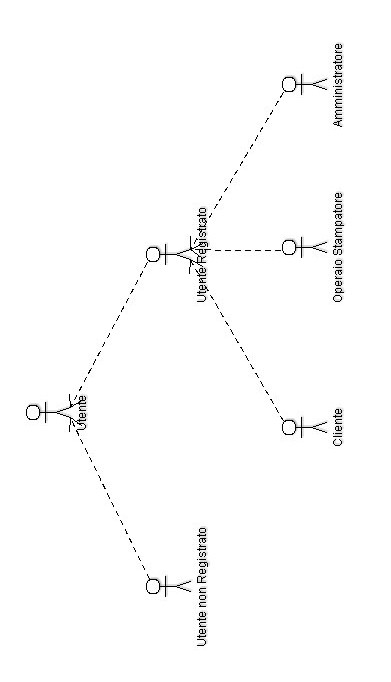
\includegraphics[height=9cm]{Immagini/GerarchiaUtenti.jpg}\\
\end{center}

\subsection{Schede dei Gruppi di Utenti}

\subsubsection{Gruppo Utente non Registrato:}
\begin{center}
	\begin{tabular}{|l|p{0.7\columnwidth}|}
		\hline
		\rowcolor[gray]{.7} \textbf{Nome Gruppo}	& \textbf{Utente non Registrato}\\
		\hline
		Descrizione & Gruppo di utenti che accedono al sito senza aver effettuato la registrazione\\
		\hline
		Dati profilo & \\
		\hline
		Super-Gruppo & \\
		\hline
		Sotto-Gruppi & \\
		\hline
		Casi d'uso rilevanti & \begin{description} 
			\item Registrazione
			\item Login
			\item Consultazione Magliette disponibili
			\item Consultazione Stampe disponibili
			\item Consultazione Pagine Informative
		\end{description}\\
		\hline
	\end{tabular}
	\begin{tabular}{|l|p{0.7\columnwidth}|}
		\hline
		Oggetti in lettura & \begin{description}
			\item Maglietta
			\item Stampa
			\item Pagina
		\end{description}\\
		\hline
		Oggetti in scrittura & Utente \\
		\hline
	\end{tabular}
\end{center}

\subsubsection{Gruppo Utente Registrato:}
\begin{center}	
	\begin{tabular}{|l|p{0.7\columnwidth}|}
		\hline
		\rowcolor[gray]{.7} \textbf{Nome Gruppo}	& \textbf{Utente Registrato}\\
		\hline
		Descrizione & Gruppo di utenti che accedono al sito con delle credenziali quali username e
		password, opportunamente definite in una precedente registrazione.\\
		\hline
		Dati profilo & \begin{description}
			\item Username
			\item Password
		\end{description}\\
		\hline
		Super-Gruppo & \\
		\hline
		Sotto-Gruppi & \begin{description}
			\item Cliente
			\item Operaio Stampatore
			\item Amministratore
		\end{description}\\
		\hline
		Casi d'uso rilevanti & \begin{description}
			\item Logout
			\item Modifica Account
		\end{description}\\
		\hline
		Oggetti in lettura & \\
		\hline
		Oggetti in scrittura & Utente\\
		\hline
	\end{tabular}
\end{center}

\subsubsection{Gruppo Cliente:}
\begin{center}
	\begin{tabular}{|l|p{0.7\columnwidth}|}
		\hline
		\rowcolor[gray]{.7} \textbf{Nome Gruppo}	& \textbf{Cliente}\\
		\hline
		Descrizione & Gruppo di utenti che accedono al sito in qualit� di clienti e pertanto hanno la
		possibilit� di acquistare i prodotti offerti dall'azienda\\
		\hline
	\end{tabular}
\end{center}
\begin{center}
	\begin{tabular}{|l|p{0.7\columnwidth}|}
		\hline
		Dati profilo & \begin{description}
			\item Nome
			\item Cognome
			\item Indirizzo
			\item Telefono
			\item Codice Fiscale
			\item E-mail
		\end{description}\\
		\hline
		Super-Gruppo & Utente Registrato\\
		\hline
		Sotto-Gruppi & \\
		\hline
		Casi d'uso rilevanti & \begin{description}
			\item Personalizzazione dei Prodotti / Magliette
			\item Modifica - Conferma Carrello
			\item Aggiunta prodotto al Carrello
			\item Visione del Dettaglio dell'Ordine
			\item Annulla Ordine
			\item Consultazione Pagine di Informazione
		\end{description}\\
		\hline
		Oggetti in lettura & \begin{description}
			\item Maglietta
			\item Stampa
			\item Pagina
		\end{description}\\
		\hline
		Oggetto in scrittura & \begin{description}
			\item Personalizzazione
			\item Riga Ordine
			\item Ordine
			\item Stampa
		\end{description}\\
		\hline
	\end{tabular}
\end{center}

\subsubsection{Gruppo Operaio Stampatore:}
\begin{center}
	\begin{tabular}{|l|p{0.7\columnwidth}|}
		\hline
		\rowcolor[gray]{.7} \textbf{Nome Gruppo}	& \textbf{Operaio Stampatore}\\
		\hline
		Descrizione & Gruppo di utenti che operano per l'azienda soddisfando gli ordini dei clienti\\
		\hline
		Dati profilo & \\
		\hline
		Super-Gruppo & Utente Registrato \\
		\hline
		Sotto-Gruppo & \\
		\hline
		Casi d'uso rilevanti & \begin{description}
			\item Prendere in carico un ordine
			\item Conferma spedizione dell'ordine
		\end{description}\\
		\hline
		Oggetti in lettura & \begin{description}
			\item Maglietta
			\item Stampa
			\item Personalizzazione
			\item Riga Ordine
		\end{description}\\
		\hline
		Oggetti in scrittura & Ordine\\
		\hline
	\end{tabular}
\end{center}
		
\subsubsection{Gruppo Amministratore:}
\begin{center}
	\begin{tabular}{|l|p{0.7\columnwidth}|}
		\hline
		\rowcolor[gray]{.7} \textbf{Nome Gruppo}	& \textbf{Amministratore}\\
		\hline
		Descrizione & Utente interno dell'azienda che si occupa della gestione degli account degli altri
		utenti registrati, dirige la gestione del catalogo (inserimento, modifica, cancellazione
		prodotti) e delle pagine informative. Pu� inoltre visualizzare il dettaglio di tutti gli 
		ordini inseriti nel sistema.\\
		\hline
		Dati profilo & \\
		\hline
		Super-Gruppo & Utente Registrato\\
		\hline
		Sotto-Gruppi & \\
		\hline
	\end{tabular}
\end{center}
\begin{center}
	\begin{tabular}{|l|p{0.7\columnwidth}|}
		\hline
		Casi d'uso rilevanti & \begin{description}
			\item Creazione - Modifica - Cancellazione Account Utente
			\item Inserimento - Modifica - Cancellazione Pagine Informative
			\item Inserimento - Modifica - Cancellazione Maglietta
			\item Inserimento - Modifica - Cancellazione Stampa
			\item Visualizzazione dettagli Ordine
		\end{description}\\
		\hline
		Oggetti in lettura & \begin{description}
			\item Ordine
			\item Riga Ordine
			\item Personalizzazione
		\end{description}\\
		\hline
		Oggetti in scrittuta & \begin{description}
			\item Maglietta [Inserimento - Modifica - Cancellazione]
			\item Stampa [Inserimento - Modifica - Cancellazione]
			\item Utente [Inserimento - Modifica - Cancellazione]
			\item Pagina [Inserimento - Modifica - Cancellazione]
		\end{description}\\
		\hline
	\end{tabular}
\end{center}	
		
		
\newpage
\section{Diagrammi dei Casi d'Uso}

\newpage
\section{Dizionario dei Dati}

\newpage
\section{Specifica delle Site View}

\newpage
\section{Linee guida dello Stile Grafico}

\newpage
\textbf{UTENTI}:
\begin{itemize}
	\item \textbf{Amministratore}
		\begin{itemize}
			\item gestione account operai azienda
			\item pagina degli ordini di diverso tipo:
				\begin{itemize}
					\item evasi (affidati al corriere: con ID di spedizione rilasciato dal corriere)
					\item non evasi (in stampa)
					\item non ancora gestiti
				\end{itemize}
			ogni ordine con i seguenti dati:
				\begin{itemize}
					\item data/ora dell'ordine e chi ha effettuato l'ordine
					\item data/ora presa in carico dall'operaio stampatore dell'ordine e chi lo ha
					preso in carico
					\item data/ora spedizione (affidamento al corriere)
					\item SERVIZI: data/ora di consegna dell'ordine
					\item SERVIZI: registro dei contatti con dati dell'operaio e dell'utente che ha
					effettuato l'ordine
				\end{itemize}
		\end{itemize}
	\item \textbf{Operaio Stampatore}\\
	L'operaio stampatore si occupa anche del confezionamento della maglietta da affidare al corriere.
		\begin{itemize}
			\item pagina degli ordini non ancora gestiti da cui pu� scegliere un ordine da prendere 
			in carico (pu� per� avere pi� di un ordine in carico)
			\item pagina degli ordini che ha in carico (operazione di: chiusura dell'ordine e di evasione
			ordine (affido al corriere))\\
			SERVIZI: ID spedizione dal corriere 
			\item ? annullamento dell'ordine da parte dell'operaio per problemi ? [vedere se mettere 
			anche questo]
		\end{itemize}
	\item \textbf{Utente Registrato}
		\begin{itemize}
			\item pagina del catalogo dei prodotti e pagine che visualizza anche l'utente non registrato
			\item pagina creazione/personalizzazione della maglietta (? multiordine ? [vedere se mettere
			questo]
			\item pagina della lista degli ordini effettuati e stato ordine con contenuti
			\item pagina di annullamento dell'ordine fino a che non � stato preso in carico dall'operaio
			\item SERVIZI: modulo di contatto utente - operaio stampatore anonimo l'uno con l'altro,
			ma l'amministratore pu� vedere, per eventuali problemi
		\end{itemize}
	\item \textbf{Utente: Home Page}
		\begin{itemize}
			\item pagina del catalogo dei prodotti
			\item pagina per la possibilit� di registrazione
			\item pagina di presentazione dell'azienda: chi siamo, dove siamo, cosa facciamo
			\item pagina di informazioni sulle spedizioni genericamente: tempi di spedizioni, costi 
			di spedizione
		\end{itemize}
\end{itemize}

Il pagamento delle magliette avviene solamente Cash al corriere.

Poi vediamo cosa aggiugere di altro in base a cosa ci dice il Profe.

\end{document}
